\begin{tikzpicture}%
\begin{scope}
\clip (1, .5) -- (.5, 1) -- (.5, 6.5) -- (.7, 6.7) -- (.7, 7.1) -- (1.2, 7.1) -- (1.2, 7) -- (7.3, 7) -- (7.3, .5) -- cycle ;
\node[anchor=south west,inner sep=0] at (0,0) {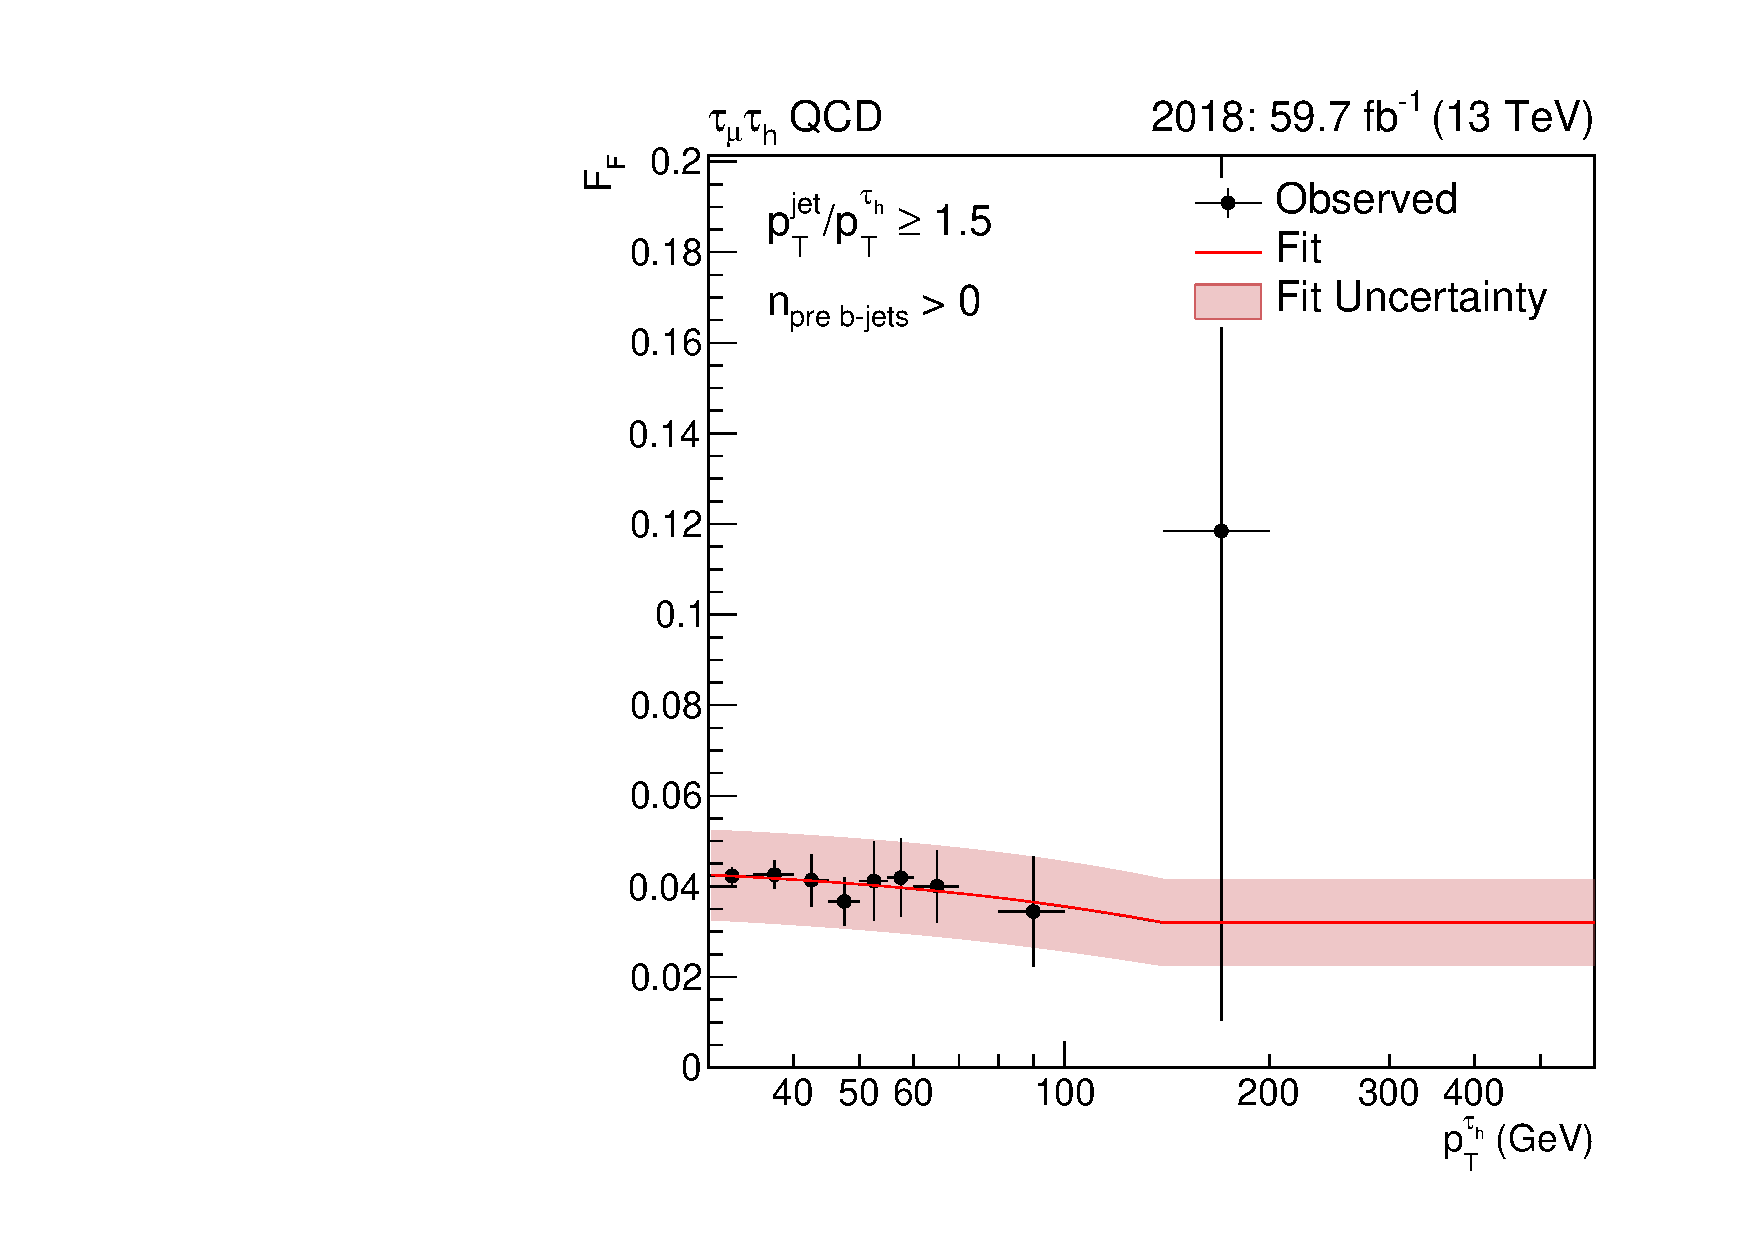
\includegraphics[width=8cm]{\PhDthesisdir/plots_and_images/from_CMS-NOTE-2020-218/ff_fit_jet_pt_high_1jet_pt_2_ff_qcd_mt_2018.pdf}};
\end{scope}

% year
\draw (7.35, 6.85) node [above left] {\scriptsize \SI{59.7}{\femto\barn^{-1}} (2018, \SI{13}{\TeV})\vphantom{Àq,}};

% category
\draw (1.1, 6.85) node [above right] {\scriptsize \mu\tauh, DR QCD};

% X axis label
\draw (7.2, -.1) node [above left] {\footnotesize $\pT^{\tauh}$ (\SI{}{\GeV})\vphantom{Àq,}};

% Y axis label
\draw (.15, 7.2) node [below left, rotate=90] {\footnotesize $\FF_Q$\vphantom{Àq,}};
\end{tikzpicture}